\documentclass[style=upen, size=14pt]{powerdot}
\usepackage{natbib}
\usepackage{bibentry}
\usepackage{mathtools}
\definecolor{arany}{RGB}{255,242,0}
\hypersetup{backref=page}
\hypersetup{
    colorlinks=true,
    linkcolor=cyan,
    citecolor=cyan,
    filecolor=magenta,      
    urlcolor=cyan}
% \pdsetup{trans=Split}
\usepackage{graphicx}
\usepackage{amsmath}
\DeclareMathOperator*{\argmax}{argmax}
\DeclareMathOperator*{\argmin}{argmin}
\DeclareMathOperator*{\softmax}{softmax}
\DeclareMathOperator{\sign}{sign}
\usepackage{graphicx,wrapfig,lipsum}
\usepackage{amssymb}
\usepackage{stmaryrd}
\usepackage[latin2]{inputenc}
%\usepackage[magyar]{babel}
%\usepackage{euler}
\usepackage{tikz}
\usetikzlibrary{matrix}
\usepackage{tikz-qtree}
\usepackage{tikz-dependency}
\usepackage{linguex}
\usepackage{amsthm}
\usepackage{amsmath}
%\tikzset{every tree node/.style={align=center,anchor=north}}
%\usepackage{tabularx}
%\usepackage{threeparttable}
%\usepackage{color}
%\selectlanguage{english}
%\frenchspacing
\usepackage{algpseudocode}
\usepackage{algorithm}
\newcommand\varlist{,\makebox[1em][c]{.\hfil.\hfil.},}
\newcommand{\nd}{\noindent}
\newcommand{\Val}{\mathop{\mathit{Val}}}
\newcommand{\gold}{\color{arany}}
%\usepackage{tikz}
%\usepackage{tikz-qtree}
%\newcommand{\qed}{\hfill\mbox{\raggedright \rule{.1in}{.1in}}}
\def\es{\mathbin\land}
\theoremstyle{definition}
\newtheorem*{definition}{Definition}
\newtheorem{axioma}{Axiom}
\newtheorem{tetel}{Theorem}
\newtheorem{prop}{Proposition}
\newtheorem{lemma}{Lemma}
\begin{document}

\title{Natural Language Processing\\~~\\Lecture 7\\Lexical semantics and\\ Latent
  Semantic Analysis}
% \author{}

\date{2021}
\maketitle

\begin{slide}{Word meanings}
  As we have seen (in Lecture 1), according to the \emph{\gold principle of
    compositionality},\medskip
  
  \emph{The meaning of a complex expression is determined by the meanings of its
    constituent expressions and the rules used to combine them.}
  \footnote{\href{https://en.wikipedia.org/wiki/Principle_of_compositionality}{Wikipedia:
      Principle of Compositionality.}}\medskip

  Although the principle is not without its problems,\footnote{See, e.g.,
    \cite{sep-compositionality}.} it suggests that to know the meaning of larger
  textual units (sentences, paragraphs etc.) it is necessary to know the
  \emph{\gold meaning of words} they are composed of.
\end{slide}

\begin{slide}[toc=]{Word meanings cont.}
  Intuitively, several words have more than one meanings, e.g. \emph{mouse} has
  a different meaning in\bigskip

  \emph{A {\gold mouse} ate the cheese.}\medskip
  
  and in\medskip

  \emph{Click on the close button with the {\gold mouse}.}\bigskip

  \emph{mouse} can mean a \emph{type of small rodent} or \emph{an electronic
    pointing device}. The identification and characterization of word meanings
  or \emph{\gold word senses} such as these is the task of \emph{\gold lexical
    semantics}.
\end{slide}


\begin{slide}[toc=Dictionaries]{Word senses in dictionaries}
  One way of characterizing word senses is offered by traditional \textit{\gold
    dictionaries}. E.g., the online version of the
  \href{https://www.oxfordlearnersdictionaries.com/definition/english/mouse_1?q=mouse}{\emph{Oxford
      Advanced Learner's Dictionary}} describes these senses as\bigskip
  
  \begin{centering}
    
    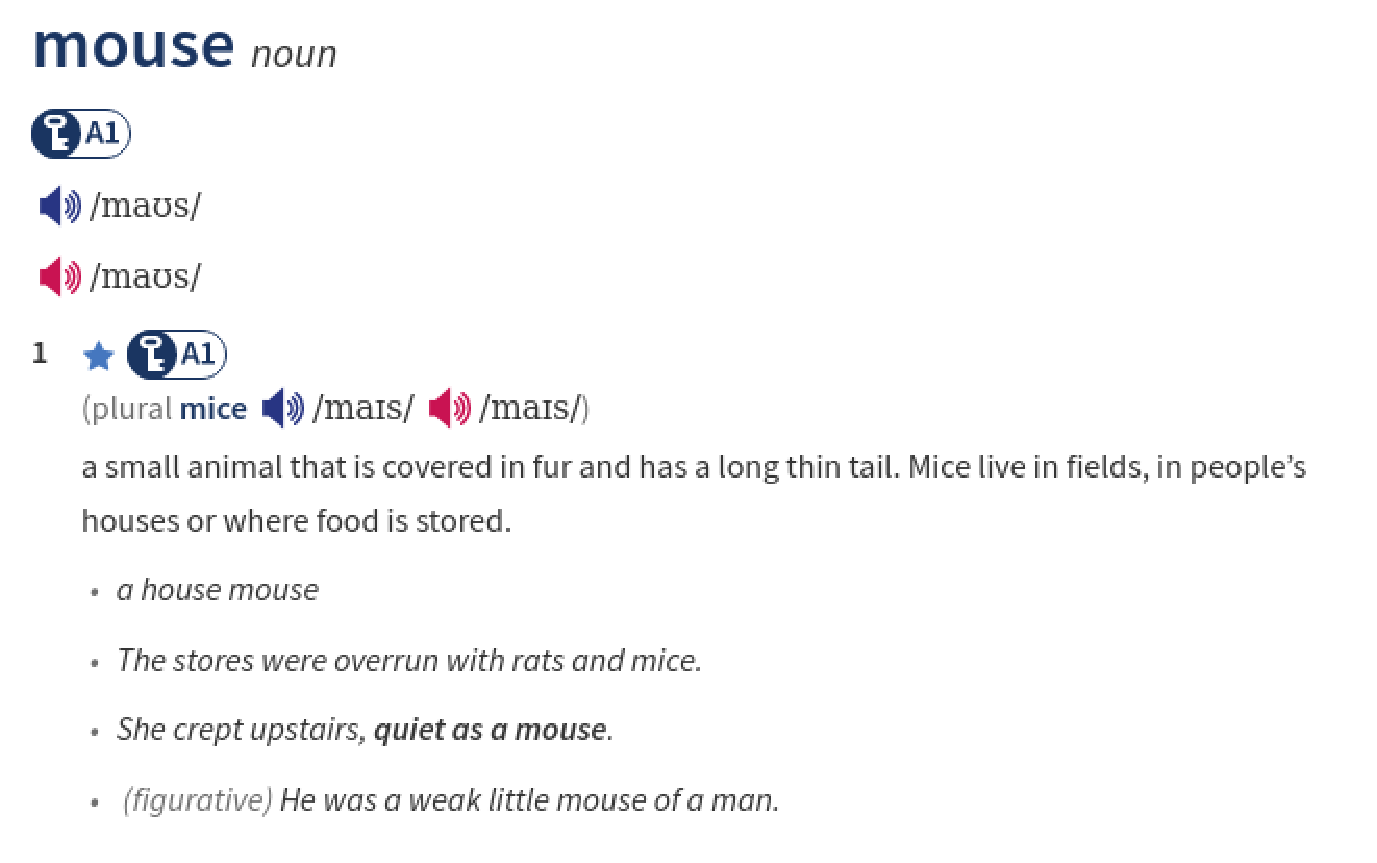
\includegraphics[width=0.75\textwidth]{figures/oald_mouse1.eps}
    
  \end{centering}
\end{slide}

\begin{slide}[toc=]{Word senses in dictionaries cont.}
  and
  
    \begin{centering}
    
    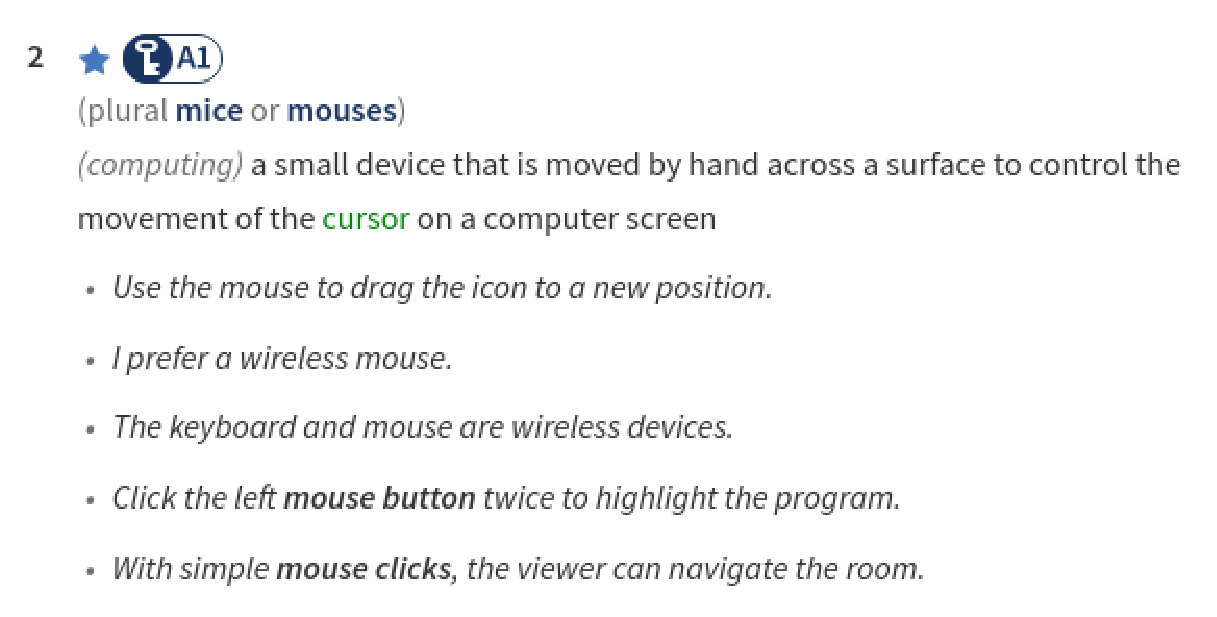
\includegraphics[width=0.8\textwidth]{figures/oald_mouse2.eps}
    
  \end{centering}

\end{slide}

\begin{slide}[toc=]{Word senses in dictionaries cont.}
  Notable features of these sense descriptions are that
  \begin{itemize}
  \item word senses have precise identifiers: the surface form \emph{mouse}, the
    POS-tag \emph{noun} and the sense number together unambiguously identify the
    senses;
  \item each sense has a \emph{\gold textual definition} which is not formal,
    but
    \begin{itemize}
    \item uses a relatively small definitional vocabulary,
    \item follows certain conventions, e.g., starts with a more general word
      plus characteristic property (\emph{small animal}, \emph{small device});
    \end{itemize}
  \item there are several \emph{\gold example sentences} illustrating typical
    patterns in which the sense is used.
  \end{itemize}
\end{slide}

\begin{slide}[toc=Lexical relations]{Lexical relations}
  Dictionaries may contain information about \emph{\gold lexical relations}
  between senses, especially about
  \begin{itemize}
  \item \emph{\gold synonymy}: whether two word senses are (close to) identical;
  \item \emph{\gold antonimy}: whether two word senses are opposites of each other.
  \end{itemize}
  Other important lexical relations include \emph{\gold taxonomical relations}:
  \begin{itemize}
  \item sense $s_1$ is a \emph{\gold hyponym} of $s_2$ if it is strictly more
    specific, e.g. \emph{mouse$_1$} is a hyponym of \emph{animal$_1$};
  \item conversely, sense $s_1$ is a \emph{\gold hypernym} of $s_2$ if $s_2$ is
    more specific than $s_1$.
  \end{itemize}
\end{slide}

\begin{slide}[toc=]{Lexical relations cont.}
  And, finally, \emph{\gold meronymy}, the \emph{part-whole} relation: e.g.,
  \emph{finger} is a meronym of \emph{hand}.\bigskip

  Collectively, word senses and their lexical relations constitute a \emph{\gold
    network}, in which
  \begin{itemize}
  \item nodes are sets of synonymous word senses, and
  \item edges are lexical relations. 
  \end{itemize}
  Since the hyponymy relation (also called \textit{is\_a}) is transitive, it
  makes sense to have only \emph{direct hyponymy} edges in the network, i.e.,
  the have an $s_1 \xrightarrow{is\_a} s_2$ edge only if there is no node $s_3$ for which
  $s_1 \xrightarrow{is\_a} s_3$ and $s_3 \xrightarrow{is\_a} s_2$.
\end{slide}

\begin{slide}[toc=WordNet]{WordNet}
  To be usable for NLP purposes, lexical semantic information has to be
  accessible as a computational resource with a well defined query API, and,
  starting from the mid. 1980s a number of projects developed such
  resources.\bigskip
  
  The most important has been the
  \href{https://wordnet.princeton.edu/}{\emph{WordNet}} English lexical
  database, which contains a large number of synonym sets with definitions,
  examples and lexical relations. After its success, WordNets were developed for
  a large number of other languages, now more than 200 WordNets are available.
\end{slide}

\begin{slide}[toc=]{WordNet cont.}
  A part of the English WordNet network:\medskip
  
  \begin{centering}
    
    \includegraphics[width=0.9\textwidth]{figures/wn.eps}


    \footnotesize{(Figure from \cite{navigli2009word}.)}
    
  \end{centering}
\end{slide}


\begin{slide}[toc=Knowledge bases]{Knowledge bases as lexical resources}
  In addition to dedicated lexical databases, \emph{knowledge bases} can also
  serve as useful lexical semantic resources, since they contain information
  about \emph{entities} and \emph{concepts}, which can be linked to words in a
  vocabulary. Important examples include
  \begin{itemize}
  \item \emph{Wikis}, most importantly the English Wikipedia, here various types
    of links and references between the entries provide relational information;
  \item \emph{formal ontologies}: these describe relationships between concepts
    in a formal logical language.
  \end{itemize}
\end{slide}

\begin{slide}[toc=WSD]{Word sense disambiguation}
  To use the information about word senses provided by these lexical resources,
  NLP applications must be able to determine in which sense words are used in
  the input, i.e., perform \emph{\gold word sense disambiguation (WSD)}.
  The details of the WSD task depend on which lexical resource it is based on
  and how the resource is used. Given a resource containing word senses, 

  \begin{itemize}
  \item \emph{\gold supervised WSD} uses machine learning methods on training data
    which is annotated with the correct word senses; while
  \item \emph{\gold knowledge-based WSD} exploits the information in the lexical
    resource, e.g. the lexical relations and definitions in WordNet.
  \end{itemize}
\end{slide}

\begin{slide}[toc=Word vectors]{Vector-based lexical semantics}
  The lexical semantic approach we have seen so far has certain features that
  make it difficult to achieve large coverage and adapt to new languages or
  domains:
  \begin{itemize}
  \item the lexical databases were manually assembled by highly qualified
    experts;
  \item the development of high-performance WSD modules typically requires a
    large amount of expert-annotated training data.
  \end{itemize}
  These problems led to research into alternatives that assign useful word
  meaning representation in an \emph{\gold unsupervised} fashion, simply
  learning them from text corpora.
\end{slide}

\begin{slide}[toc=]{Vector-based lexical semantics cont.}
  Although there have been attempts to learn \emph{semantic networks} from text
  corpora, the first successful unsupervised lexical semantic methods have been
  learning \emph{\gold word vectors} from text corpora, i.e., embedding
  functions of the form
  $$
  E: V \rightarrow R^d
  $$
  which assign $d$-dimensional ($d\in \mathbb N$) vectors to each word in the
  $V$ vocabulary. Of course, not any such function will do: the obvious
  requirement is that the learned vectors has to convey useful information about
  the \emph{meaning} of the words they are assigned to.
\end{slide}

\begin{slide}[toc=]{Vector-based lexical semantics cont.}
  One way of ensuring the connection is to utilize the \emph{distributional hypothesis}:
  \begin{itemize}
  \item ``You shall know a word by the company it keeps.''
    \footnote{J.R. Firth, \emph{Papers in Linguistics 1934--1951 (1957).}}
  \item ``Linguistic items with similar distributions have similar meanings.''
    \footnote{\href{https://en.wikipedia.org/wiki/Distributional_semantics}{Wikipedia:
        Distributional semantics.}}
  \end{itemize}
  This suggests that if the word vectors reflects the \emph{distribution} of the
  words they are assigned to, then they will also reflect the words' meanings.
\end{slide}

\begin{slide}[toc=]{Co-occurrence matrices}
  The most direct way of getting word vectors that reflect the words'
  distribution in a corpus is to consider \emph{co-ocurrence} matrixes. If there
  are $D$ documents in the corpus and $V$ is the corpus vocabulary then
  \begin{itemize}
  \item \emph{\gold term-document} matrices are $|V|\times D$ dimensional
    matrices in which each row is a word vector whose $i$-th element is the
    occurrence count of the word in the $i$-th document, while
  \item \emph{\gold term-term} matrices are $|V|\times |V|$ dimensional matrices
    in which each row is a word vector whose $i$-th element is the co-occurrence
    count of the word with the $i$-th \emph{other word}.
  \end{itemize}
\end{slide}

\begin{slide}[toc=LSA]{Latent Semantic Analysis}
  An important problem of using these vectors directly is their huge
  dimensionality and sparsity. To solve this problem, \emph{\gold Latent
    Semantic Analysis} methods apply dimension reducing matrix factorization
  methods, typically \emph{truncated SVD} to find a \emph{low-rank
    approximation} of the original $C$ co-occurrence matrix. With SVD the factorization is
  $$
  C = USV^\intercal
  $$
  with $U,V$ orthonormal and $S$ diagonal. In case of truncated SVD, the rows of
  the $U$ matrix can be used as low-dimensional, approximate representations of
  the co-occurrence based original word vectors.
\end{slide}

\begin{slide}{References}
  \bibliographystyle{plainnat}
  \nobibliography{nlp_course.bib}
  \begin{footnotesize}

    \bibentry{sep-compositionality}.\medskip

    \bibentry{navigli2009word}.\medskip

  \end{footnotesize}
\end{slide}

% \begin{slide}[toc=]{References cont.}
%   \begin{footnotesize}

%     \bibentry{peters2018deep}.\medskip
    
%   \end{footnotesize}
% \end{slide}

\end{document}

%%% Local Variables:
%%% mode: latex 
%%% TeX-master: t
%%% End:

% LocalWords:  Tokenization Discriminative discriminative
